79.  $f(x)=\cfrac{|x^2+2x|(x-1)}{x}=\cfrac{|x||x+2|(x-1)}{x}=\begin{cases} x^2+x-2,\ x>0,\\ -x^2-x+2,\ -2<x<0,\\ x^2+x-2,\ x\leqslant-2.\end{cases}$
$$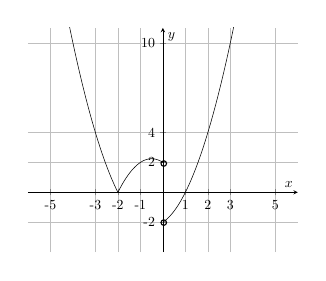
\begin{tikzpicture}[scale=0.5]
\begin{axis}[
    axis lines = middle,
    grid=major,
    legend pos={south west},
    xlabel = {$x$},
    %xlabel style={below right},
    ylabel = {$y$},
    ymin=-4,
    ymax=11,
    xmin=-6,
    xmax=6,
    xtick={-5,-3,-2,-1,1,2,3,5},
    xticklabels={-5,-3,-2,-1,1,2,3,5},
    ytick={10,2,-2,4},
    yticklabels={10,2,-2,4},
                  ]
	\addplot[domain=-6:0, samples=100, color=black] {-abs(x+2)*(x-1)};
    \addplot[domain=0:6, samples=100, color=black] {abs(x+2)*(x-1)};
        %\addplot[domain=2.01:6, samples=100, color=black] {2/(2-x)};
   % \addplot[domain=-3:3, samples=100, color=black] {-x};
     %\addlegendentry{$\text{Рис. 1}$};
\end{axis}
\draw (3.45,2.25) circle (2pt);
\draw (3.45,0.75) circle (2pt);
%\draw (3.45,2.55) circle (2pt);
\end{tikzpicture}$$
